

\subsection{Molecular Dynamics (MD)}
Due to the high charge states seen in experiment with clusters the only
practical method to microscopically study the ionization dynamics is
\textit{Molecular Dynamics} (MD) methods where ions and electrons are treated
classically.

In MD, particles interact directly through classical instantaneous forces. The
total force acting on particle $i$ of mass $m_i$ from all other $N$ particles in
the system is:
\begin{align}
m_i \va_i & = \vF_i = \sum_{j \ne i} \vF_{j \rightarrow i}
\label{eqn:md:newton}
\end{align}
In the present work, the force between charged particles is the instantaneous
electrostatic Coulomb force:
\begin{align}
\vF_{C,j \rightarrow i}\pa{\vr} & =\frac{k q_i q_j}{r_{ji}^2} \hvr_{ji}.
\label{eqn:md:coulomb:F}
\end{align}
which only depends on the distance between particles. Figure
\ref{fig:md:vectors} shows the vectors definition used throughout this work. We
define particle $i$ the particle we are interested in (for example, the
particle we are calculating the force on), and particle $j$ the particle that
is generating the field or potential that is measured at location $i$. We thus
have:
\begin{align}
\vr_{j} + \vr_{j,i} & = \vr_{i} \\
\vr_{j,i} & = \vr_{i} - \vr_{j}
\end{align}
%       _j
%       /|\
%  r_j /   \ r_ji
%     /    _\/
%    /------>i
%       r_i

\emptyfig{Vectors definition}{fig:md:vectors}


Equation \eqref{eqn:md:newton} can be time integrated using the
Velocity-Verlet (VV) scheme:
\begin{subequations}
\begin{align}
\vx_{i}^{\pa{n+1}} & = \vx_{i}^{\pa{n}} + \vv_{i}^{\pa{n}} \Delta t +
\frac{\va_{i}^{\pa{n}}}{2} \Delta t^2, \\
\va_{i}^{\pa{n+1}} & = \frac{\vF^{\pa{n}}}{m_i} \label{eqn:md:vv:a} \\
\vv_{i}^{\pa{n+1}} & = \vv_{i}^{\pa{n}} + \frac{\va_{i}^{\pa{n}} +
\va_{i}^{\pa{n+1}}}{2} \Delta t,
\end{align}
\label{eqn:md:vv}
\end{subequations}
where $\Delta t$ is the integration time step, $\vx_{i}$ the position vector,
$\vv_{i}$ the velocity vector and $\va_{i}$ the acceleration vector of
particle $i$, all evaluated at either the time step $n$ or the next one $n+1$.
Equations \eqref{eqn:md:vv}, when applied to every particles $i$ of the system,
can thus be used to propagate in time the whole cluster. Note that many
variation of equations \eqref{eqn:md:vv} are possible but all are equivalent.

Every particle in the system stores its position $\vx^{\pa{n}}$, its velocity
$\vv^{\pa{n}}$ and also the total force acting on it $\vF^{\pa{n}}$. This total
force is the sum of all contribution of equation \eqref{eqn:md:coulomb:F} from
all other particles in the system.

The MD algorithm basically calculates the force between every pair of particles
in the system. Since there is $N$ total particles, there is $O\pa{N^2}$
interactions to calculate. Doubling the number of particles will quadruple the
computational burden, effectively putting an upper limit on the number of
particles that can be simulated to tens of thousands.

\subsection{Long range potential: Hierarchical Tree algorithms}
The $O\pa{N^2}$ scaling of MD algorithm can be problematic when the number of
particles simulated is more than many thousands, which is a potential target
for laser-cluster interaction. Some interesting variations of the MD algorithm
exist to reduce the computational burden. These \textit{hierarchical tree}
algorithms were introduced\cite{Barnes1986} by Barnes and Hut in 1986. To
reduce the computational burden, particles are grouped in a hierarchical tree
(quadtree in two dimensions, octree in three). While Barnes used his
\textit{treecode} to solve the N-body problem in the context of gravitational
interactions, it can also be applied in the electrostatic case.

The main issue with the direct calculation of forces in MD is the lack of
distinction between the close particles and distant ones. While the resulting
potential of a distant particle is small, the computational cost required to
calculate it is the same as in the case of a nearby particle. Some MD
calculation use an artificial cutoff; particles farther then this cutoff will
be ignored in the calculation of the force on one particle. This is acceptable
when the force acting on particles is short range, either due to screening or
to the nature of the force. In the present work, the dominant force is the
Coulomb force and is a long range one by nature; it thus cannot be artificially
cutoff as in the case of close range forces used in other fields.

Could distant particles be grouped together, with their contribution to the
force (or potential) being calculated only once (per ``group'')? Because
individual particles which are part of a distant group will have a similar
contribution to the potential at the location of particle $i$, the interaction
with this group can be instead approximated through the multipole
expansion\cite{Gibbon2002} of the group of particles, or cell in terms of the
tree algorithm:
\begin{align}
\phi_i & = \sum_{j~\textrm{cell}} \phi_{j \rightarrow i} = \sum_{j~{\rm cell}}
\frac{k q_j}{r_{ji}} \\
& \approx \frac{M_{c}}{R}
+ \sum_{\alpha} \frac{r_{\alpha} D_{c,\alpha}}{R^3}
+ \frac{1}{2} \sum_{\alpha,\beta} \frac{
        Q_{c,\alpha,\beta} r_{\alpha} r_{\beta}
    }{R^5}
\end{align}
where $M_{c}$, $D_{c,\alpha}$ and $Q_{c,\alpha,\beta}$ are the monopole, dipole
and quadrupole moments of the cell defined as:
\begin{subequations}
\begin{align}
M_{c}           ~~~~& = \sum_{j~\textrm{cell}} q_{j} \\
D_{c,\alpha}      ~~& = \sum_{j~\textrm{cell}} q_{j} r_{j,\alpha} \\
Q_{c,\alpha,\beta}  & = \sum_{j~\textrm{cell}} q_{j} \pa{3 r_{j,\alpha}
r_{j,\beta} - r_{j}^2} \delta_{\alpha,\beta}
\end{align}
\label{eqn:tree:moments}
\end{subequations}
and $R$ is the distance between the cell's centre-of-charge and the
particle of interest $i$.

\emptyfig{QUAD TREE}{fig:tree:quadtree}

The tree algorithm first split the computational domain into a quadtree until
only a maximum of one particle is present per cell. The tips of the tree,
containing only one particle, are called leaves. Once every particles in the
system are inserted in the tree, the electrostatic moments are propagated from
the leaves up to the root cell, the top cell enclosing the whole domain.

Then, instead of iterating through all particles for the calculation of the
force on the particle of interest $i$, the tree is traversed. If the cell is
``far enough'' (with a given definition of far enough, discussed next) it can
be added to the a cell interaction list for later processing. In the case of
the cell being to close, it must be resolved into its  eight \textit{daughter}
cells. The daughter cells containing particles are visited, while the empty
ones are ignored. The leaf cells can be reached using this process; in this
case, the particles in the leaves are considered close enough to the particle
of interest $i$ and a direct interaction is wanted. The leaf particle will thus
be added to a second interaction list containing particle-particle direct
interactions. The process is recursively repeated until all particles
are added to an interaction list, either directly or through a parent cell.

Different selection rules exist for the criteria of ``far enough''. These
rules are called \textit{Multipole Acceptance Criteria} or
MAC\cite{Pfalzner1996}. Barnes' original one simply referred as
``\textit{s/d}'' compares an input parameter $\theta$ with the cell's size $s$
divided by the distance between the cell's center-of-charge and particle of
interest $i$. If the ratio $s/d$ is smaller than the parameter $\theta$, the
group of particles contained inside the cell is approximated through the cell's
moments and the cell is added to the cells interaction list. At the opposite, if
the ratio is larger than $\theta$, the cell will be resolved into its daughters.
In the limit where $\theta$ reaches zero, no more cells are added to the
cells interaction list (they are all resolved) and the MD algorithm emerges.

Unfortunately, this MAC can cause huge errors when large amount of charge is
present in a corner of a cell. In this case, a cell could be added to the cell
interaction list even though the error introduced by the multipole expansion is
significant. Different MAC have thus been proposed to mitigate this problem.
The \textit{minimum distance} MAC replaces the distance $d$ in the MAC with the
minimum distance to one of the cell's edge. The \textit{B-max} MAC instead
replaces the size of the cell with the largest distance between one of the
cell's corner to the center-of-charge. Another MAC was proposed by Bédorf
\textit{et. al.} \cite{Bedorf2012} and is a mix of the two previous. The MAC
reads:
\begin{align}
d > \frac{s}{\theta} + \delta
\end{align}
where $\delta$ is the distance between the cell's geometric center and its
center-of-charge. If the previous equation holds ($d$ is large enough) then the
multipole expansion is used; the cell is added to the interaction list.

The different MAC can be seen on figure \ref{fig:tree:mac}.

\emptyfig{MAC DIAGRAM}{fig:tree:mac}

Because not all interaction pairs are considered in the calculation of the
force and potential, a significant speedup is obtained. Due to the tree
traversal algorithm, the scaling passes\cite{Barnes1986,Gibbon2002,Pfalzner1996}
from $O\pa{N^2}$ to $O\pa{N \ln{N}}$.

A variation to the hierarchical treecode is obtained when a sufficiently large
$\theta$ is used. In this case, the root cell (the largest one) is never
resolved into its daughters. By adding more moments to the approximation then
the first three ones of equations \eqref{eqn:tree:moments} and removing
contributions of nearby particles, the \textit{Fast Multipole Method} (FMM) is
obtained\cite{Pfalzner1996}. FMM was developed by Greegard in
1988\cite{Greengard1987} independently of Barnes' hierarchical tree method.
While conceptually similar, its implementation details are quite different and
has not been implemented in the current work.

\emptyfig{TREECODE SCALING}{fig:tree:scaling}




\subsection{Short range potential: shapes}
\label{section:intro:md:potentials}

An important problem to consider is the close range behaviour of equation
\eqref{eqn:md:coulomb:F} which diverges. Additionally, electrons should not be
able to classically recombine to an ion under the atomic energy level. To
prevent the later, electron recombination, as described in section
\ref{section:intro:clusters:heating}, can be enabled. But this does not prevent
the divergence of the Coulomb force. Instead, the problem is resolved by
changing the shape of equation \eqref{eqn:md:coulomb:F} at close range.
Different \textit{smoothing potentials} can be used to prevent the
discontinuity of the Coulomb potential (or force).


Different potential shapes were investigated for the close range potential.
Figure~\ref{fig:potential:shapes} plots the different shapes of potentials and
their respective electrostatic field. These shapes are obtained by simply
finding the location $R$ where the value and the slope of the close-range shape
$\phi_{cr}$ fits with the Coulomb potential $\phi_C$.
\begin{subequations}
\begin{align}
\left. \phi_C        \right|_{R} & = \left. \phi_{cr} \right|_{R} \\
\left. \delr{\phi_C} \right|_{R} & = \left. \delr{\phi_{cr}} \right|_{R}
\end{align}
\label{eqn:potential:to_match}
\end{subequations}

These locations $R$ are the cutoff radius of these shapes and mark the switch
between the long range Coulomb potential and the short range potential.

\subsubsubsection{Harmonic}
For the harmonic potential, we have:
\begin{align}
\phi_{j,H} & = -A r^2 + \phi_0
\end{align}
We note that at $r_{j,i} = 0$, the potential value is the ``potential depth''
$\phi_0$.
Matching equations \eqref{eqn:potential:to_match} at $R$ gives:
\begin{subequations}
\begin{align}
\phi_{j,H}\pa{\vr_i} & = \frac{-4 \phi_0^3}{27 \pa{k q_j}^2} r_{j,i}^2 + \phi_0
\\
R & = \frac{3 k q_j}{2 \phi_0} \\
\vE_{j,H}\pa{\vr_i} & = \frac{k q_j}{R^3} \vr_{j,i}
\end{align}
\end{subequations}


\subsubsubsection{Super-Gaussian}
The super-gaussian potential is given by:
\begin{align}
\phi_{j,SG}\pa{\vr_i} & = \phi_0 \ex{
                            -\frac{1}{2} \pa{\frac{r_{j,i}}{\sigma}}^{2m}
                        }
\label{eqn:potential:shapes:sg:pot}
\end{align}
In the case where $m = 1$, equation \ref{eqn:potential:shapes:sg:pot} is simply
a gaussian shape. Matching equations \eqref{eqn:potential:to_match} at $R$ gives
values for $\sigma$ and $R$:
\begin{subequations}
\begin{align}
\sigma  & = \frac{k q_j m^{1/2m}}{\phi_0} \ex{\frac{1}{2m}} \\
R       & = \frac{k q_j}{\phi_0} \ex{\frac{1}{2m}} \\
\vE_{j,SG} & = \frac{\phi_0 m}{r_{j,i}}
                \ex{-\frac{1}{2} \pa{\frac{r_{j,i}}{\sigma}}^{2m}}
                \pa{ \frac{r_{j,i}}{\sigma} }^{2m}
                \hvr_{j,i}
\end{align}
\label{eqn:potential:shapes:sg}
\end{subequations}





\subsubsubsection{Gaussian distribution}
An efficient way is to treat electrons as charge distributions instead of point
particles. As such, the electrostatic potential due to a charge particle $j$
(of gaussian shape of width $\sigma$) at location $\vr = r \hvr$ is:
\begin{align}
\phi_{j}\pa{\vr} & = \frac{k q_j}{r} \erf{\frac{r}{\sigma \sqrt{2}}}
\label{eqn:md:smoothed:phi}
\end{align}
The associated electrostatic field is thus:
\begin{align}
\vE_{j}\pa{\vr} & = -\grad{\phi_j\pa{\vr}} = k q_j \pa{
    \frac{ \erf{\frac{r}{\sigma\sqrt{2}}} }{r^2}
    - \sqrt{\frac{2}{\pi}} \frac{ \ex{-\frac{r^2}{2 \sigma^2}} }{\sigma r}
} \hvr
\label{eqn:md:smoothed:E}
\end{align}
When the distance $r$ is large compared to $\sigma$, the error function
is close to 1 and the potential becomes Coulombic. Also, the exponential
term in the electric field will tend towards 0 (since it's a gaussian shape).
The error function will tend towards 1, so the electric field will
be the field of a discrete point charge.

The value of $\sigma$ is arbitrary: the smaller it is, the closer the potential
will be from the pure Coulomb one. We can set a value for $\sigma$ from the
extremum value of the potential which occurs at $\vr = 0$. At $\vr = 0$, an
indetermination $\frac{0}{0}$ occurs. Using l'Hospital rule, we get the limit
of $\phi$ as $\vr$ reaches 0:
\begin{align}
\lim_{\vr \rightarrow 0} \phi_j\pa{\vr}
    & \equiv \phi_j\pa{0} = \frac{ k q_j }{ \sigma } \sqrt{\frac{2}{\pi}}
\end{align}
from which we get the particle width:
\begin{align}
\sigma & = \frac{ k q_j }{ \phi_j\pa{0} } \sqrt{ \frac{2}{\pi}}.
\label{eqn:md:sigma}
\end{align}
The free parameter is thus the ``potential depth'' $\phi_j\pa{0}$. We call this
parameter ``depth'' since the potential energy of an electron on top of an ion
would be minimum, similar to the gravitational potential energy of a ball is
minimum at the bottom of a well.

Another problem that the smoothing of equations \eqref{eqn:md:smoothed:phi} and
\eqref{eqn:md:smoothed:E} solve is the one of \textit{numerical heating} which
occurs when particles artificially gain (or loose) energy during the
calculation of equations \eqref{eqn:md:vv}. This absence of conservation of
energy is due to a time step $\Delta t$ which is too large. Indeed, the
discretization of equations \eqref{eqn:md:vv}, and most importantly of
subequation \eqref{eqn:md:vv:a}, assumes the force on each particle to have a
linear variation between time steps. If the time step is too large and the
curvature of equation \eqref{eqn:md:smoothed:E} can be sampled by the moving
particle between each time steps, then the energy will not be conserved.



Figure \ref{fig:potential:shapes} show the different potential shapes and their
respective electrostatic field.

\begin{figure}
    \begin{center}
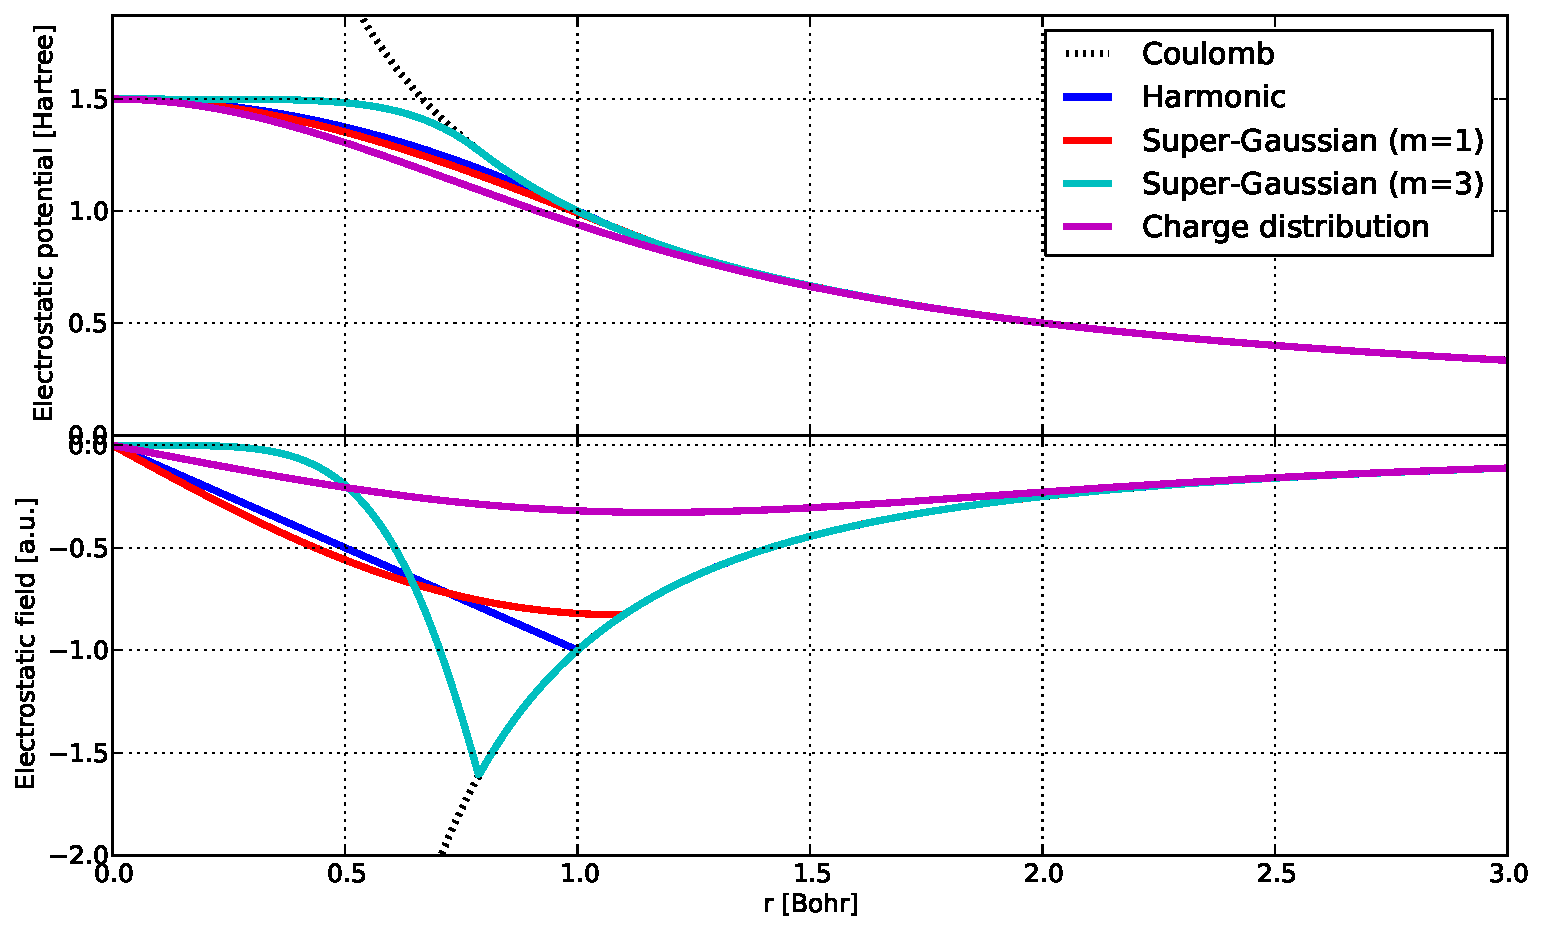
\includegraphics[width=0.98\columnwidth]{figures/potential_shapes}
    \end{center}
    \caption{\label{fig:potential:shapes}Potential shapes and their respective
electric field. Note the use of atomic units and $\phi_0$ = 1.5 Hartree.}
\end{figure}

It was found that the potential given by the charge distribution of equation
\eqref{eqn:md:smoothed:phi} and the associated electrostatic field of
\eqref{eqn:md:smoothed:E} give the less numerical heating. As explained
previously, the time discretization used to integrate the equations of motion
assume that the change in force between two time steps is linear. As can be
seen on figure \ref{fig:potential:shapes}, the charge distribution curve
(magenta) does not have a discontinuity and is therefore the prefered one.

To validate the selection of the smoothing curve, photo-ionization was forced
on a single atom and the total energy tacked. In this ionization case, the
electron comes out of the ion with a maximum of kinetic energy. It is thus a
good candidate to test if numerical heating is present or not. If the total
energy is conserved, then the selected parameters (potential depth, smoothing
curve and time step) can be used with good confidence. Figure
\ref{fig:potential:heating} shows numerical heating.


\emptyfig{NUMERICAL HEATING}{fig:potential:heating}


\subsection{Implementation details}

Our group previously used Barnes and Hut treecode implementation,
freely available\cite{treecode} through the GPL version 2. The code was adapted
to simulate charged particles (Coulomb force) instead of masses (gravitational
force) with some ionization routines added (see for example reference
\cite{Jungreuthmayer2005}). While reducing development time by re-using already
written code, the maintenance burden introduced by many factors (initial
implementation written in the C language, usage of global variables
throughout the code, multiple coding styles from different people throughout
the years, lack of vision, lack of revision control system to give the freedom
of deleting code from the active version without loosing the ability to roll
back, many subtle and important bugs, stability issues, etc.) pushed the author
to restart from scratch. This allowed using modern development techniques to be
used. For example, all development was done through a revision control system
(subversion\cite{svn} at first, then switched to git\cite{git}) in the C++
language instead of C. The object oriented nature of C++ allowed encapsulation
of different parts of the code which could then be tested and validated
individually. This gave better flexibility to the code, a required asset to
push further the development of features.

A substantial number of MD packages are freely available and were
their usage was considered instead of re-implementing a new one from scratch.
Examples are GROMACS\footnote{GROMACS:
\url{http://www.gromacs.org/}} or NAMD\footnote{NAMD:
\url{http://www.ks.uiuc.edu/Research/namd/}}. A major issue with these
pre-existing MD packages is their target audience; they aim to simulate large
bio-molecules with mostly short range interactions. Another important problem
is the number of particles throughout the simulations; while many packages
assume a constant number of particles, the present work required creating
(ionization) and annihilating (recombination) particles throughout simulations.
Controlling the MD part of the code allowed better integration of the
ionization aspects.

Other MD packages were not mature enough or simply non-existent at the time.
For example the largely used HOOMD-blue\footnote{HOOMD-blue:
\url{http://codeblue.umich.edu/hoomd-blue/}} which uses extensively
Nvidia GPUs released its first version (v0.6.0) in February 2008.
Additionally, the knowledge and experience gained by writing from scratch such
a package is invaluable.
